\section{Introduction}
%As per the Cisco Visual Networking Index (VNI) latest report (updated on February, 2019)\footnote{\url{https://www.cisco.com/c/en/us/solutions/collateral/service-provider/visual-networking-index-vni/white-paper-c11-741490.html} (\lastaccessedtoday)}, the global IP video traffic has been forecast to be 82\% of all IP traffic (both business and consumer) by 2022, which is up from 75\% as reported in 2017. Considering this heavily biased Internet traffic towards the video streaming services, new protocols and technologies are being developed for efficiently managing the quality of experience (QoE) for the streaming users. Google has developed and publicized Quick UDP Internet \blue{Connections} (QUIC)~\cite{langley2017quic} \blue{protocol} which brings up the end-to-end data transport functionalities as an application service while using UDP at the transport protocol. 
Quick UDP Internet Connection (QUIC)~\cite{langley2017quic} has been developed and experimentally deployed over the Internet by Google to replace TCP as the transport layer protocol, while addressing the limitations of TCP for end-to-end connection managements over a wide range of applications. While majority of the global Internet traffic originates from various video streaming applications, QUIC claims to reduce the YouTube rebuffering by a margin of 18\% for desktop users and 15.3\% for mobile users~\cite{langley2017quic}. As Dynamic Adaptive Streaming over HTTP (DASH)~\cite{stockhammer2011dynamic} has been a de facto for Adaptive Bitrate Streaming (ABR) over the Internet, it would be interesting to explore how QUIC performs over various ABR techniques proposed in the recent literature in terms of end users' quality of experience (QoE).

%\begin{figure}
%    \centering 
%	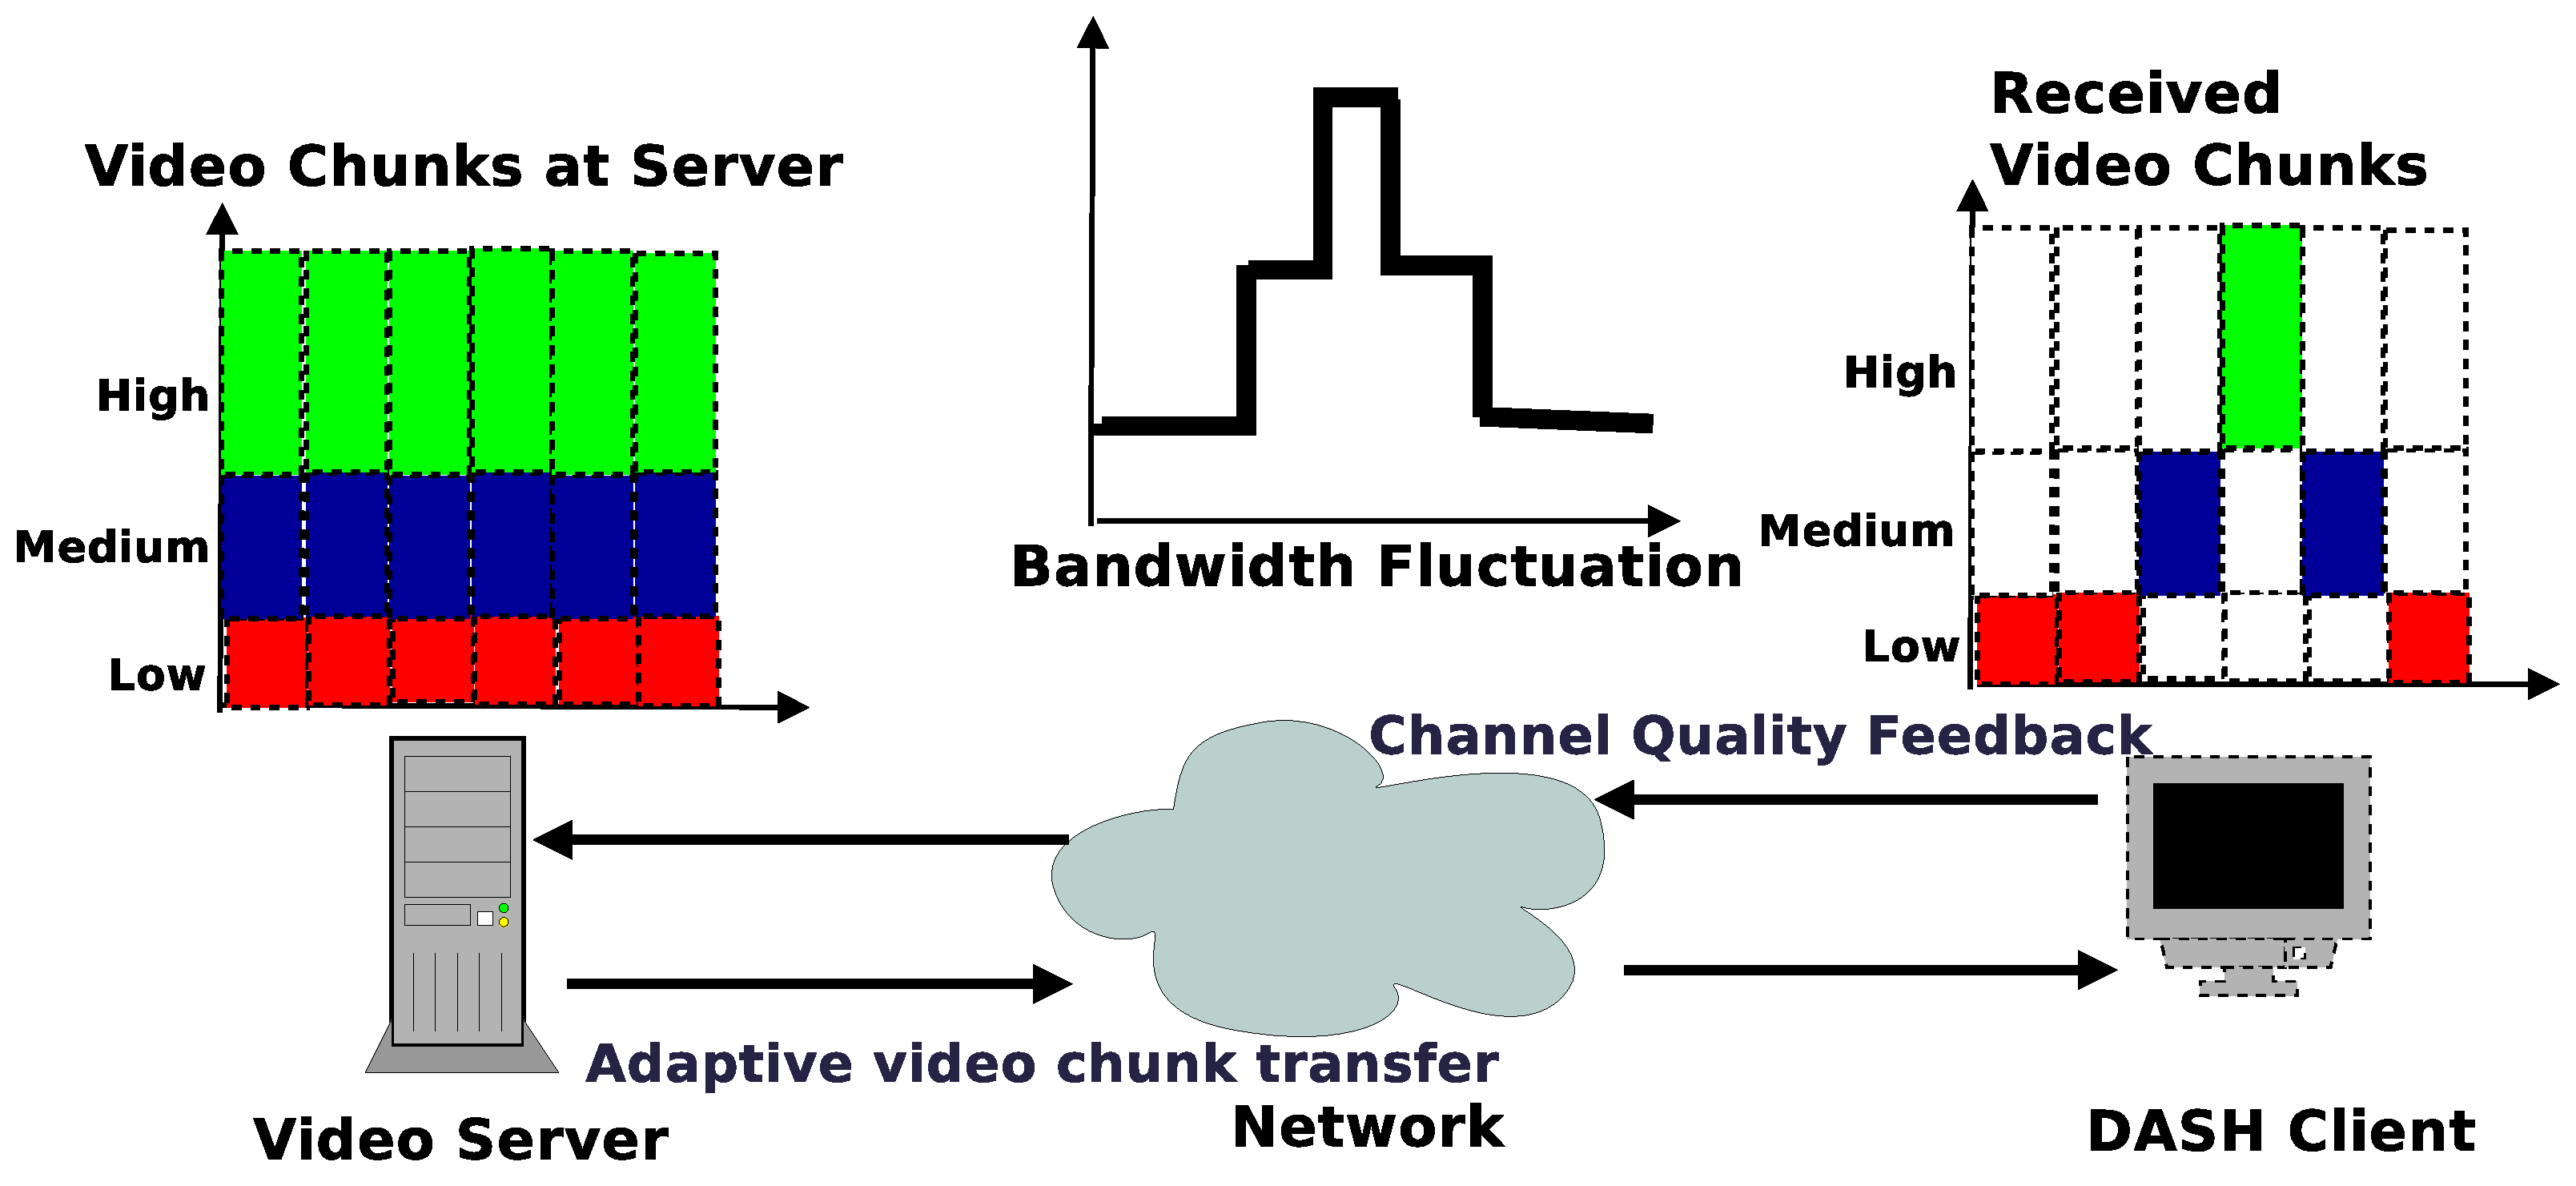
\includegraphics[width=\linewidth]{img/dash.eps}
%	\caption{\label{fig:dash} DASH based Adaptive bitrate streaming}
%\end{figure}

In DASH, the videos are divided into small segments, and every segment is encoded in multiple quality levels (bitrates). The DASH client measures the network condition and requests for a video segment with the most suited quality level based on the current network condition. The network measurement and the corresponding bitrate adaptation algorithm can be tuned in DASH, and a large number of works have been proposed in the literature to select the optimal ABR technique, such as buffer based (BOLA~\cite{bola-2016}), using control-theoretic approach (MPC~\cite{yin2015control}), or based on deep reinforcement learning (Pensieve~\cite{mao2017neural}). However, these existing approaches do not look into the impact of the underlying transport protocols on the video streaming QoE performance. While TCP uses multiple socket connections to download the video and the corresponding audio data, QUIC multiplexes the audio and the video streams over a single UDP socket to download the entire data from the server. 
%Therefore, the QUIC connections are much longer and steady compared to HTTP/TCP connections. 
As the ABR techniques depend on the channel throughput estimation at the client, such protocol changes are likely to impact the streaming performance. 


%As most of these existing approaches have pointed out, the video QoE for an adaptive bitrate streaming strategy can be quantified with the following three metrics --  While a high average playback bitrate gives a better QoE, an increased rebuffering duration or a reduced playback smoothness drops the perceived QoE level.    

With the above context, this letter evaluates and compares the performance of various ABR techniques over TCP and QUIC. We develop a testbed setup with the help of a standard DASH player from the DASH Industry Forum, where we integrate the DASH player with QUIC and use emulated network environment based on a large pool of pre-collected network traffic traces. 
%We have used a total of $45$ hours of video data from videos of different lengths, to stream over the network. To emulate bandwidth variation in the network, we have set up a traffic shaper in between the video streaming server and the DASH player; the traffic shaper emulates realistic network bandwidth behavior from a large pool of pre-collected traffic traces from the publicly available dataset. 
With a total of $45$ hours of streaming video data, we have computed three QoE metrics -- (a) average playback bitrate, (b) total rebuffering duration, and (c) playback smoothness, while streaming over both TCP and QUIC. Our thorough experiments and observations indicate that recent ABR techniques provides better QoE over TCP compared to QUIC. We investigate further to understand the protocol-level behavior of QUIC, which impacts the QoE performance.
Our analysis reported in this letter can help the community to tweak the QUIC configurations to obtain the best QoE performance from the modern ABR techniques. 
%are more compatible with TCP compared to QUIC, and new ABR techniques need to be designed to get the best performance out of QUIC. 

%Online video streaming is one of the most popular online services on the Internet. Currently, it has a majority share of the overall Internet traffic. Online video streaming gain popularity with video streaming service over the HTTP. Before HTTP based streaming service, there was RTP based video streaming. The fundamental difference between RTP and HTTP based services is that RTP uses the push mechanism where HTTP uses the pull mechanism. In case of RTP, client/player usually informs the server that it wants a particular video, and then server pushes all the video frames over the network/Internet. Here a client does not have much control over the video playback. Also, it is tough to adapt the video quality as per the network condition. As RTP uses the push mechanism, it is tough to stream to a player inside a private network.

%HTTP based streaming does not have such problems. All the video traffic are treated as HTTP traffic only. A client can be a simple browser or some dedicated player which request video from a server as a form of HTTP request and put that segment to the buffer when it gets back the requested video segment from the server. It reduce the requirement of specialized server for video streaming. A streaming provider can use normal CDN to set up video streaming. The only thing a streaming provider has to do is put multiple quality version in there CDN so that player can choose optimal quality video for a device. It saves server bandwidth as well as user's data consumption.

%At this point, a streaming video player has the option to play video from a wide variety of quality available in the server. As a player already have an option to understand the network quality by looking at the download speed while downloading each segment, it can dynamically decide what quality segment to be download next so that user can get better QoE concerning video quality and the number of stalls in the video playback. So, Dynamic Adaptive Stream over HTTP (DASH) is proposed.
%
%As per DASH, the server will keep multiple quality version of the same video in the server. A video player always monitors the network conditions and some other parameters and adapt the video quality on the fly to improve QoE. Streaming video provider like YouTube, Netflix, Amazon prime uses DASH-like architecture for there service. In Fig.~\ref{fig:dash}, standard DASH adaptation procedure is depicted.




%Now, from the network point of view, data delivery speed is very critical for streaming provider as well as other web-based service providers. A browser needs to downloads several items to render a web page. Those item needs to be downloaded individually, and each item needs different TCP socket. As those items are tiny, it is very inefficient to download multiple small items over independent TCP connection. To solve this type of problems, Google developed a new protocol Quick UDP Internet Protocol (QUIC)\cite{QUIC-2017}. It multiplexes multiple HTTP streams over single QUIC connection. It also provides 0-RTT connection establishment time which increases its performance many folds. According to Google, it also improves QoE of online video streaming. Google chrome and chromium browser implements QUIC protocol.

%In this paper, we are comparing the QoE and other parameters while a video is playing through TCP or QUIC.